\documentclass[12pt]{jarticle}
\usepackage{graphicx}
\begin{document}


  \begin{eqnarray}
    H: 1 [Oe] &=&  1000 / 4\pi[A/m] \\
    M: 1 [emu] &=& 1 / 1000 [A \times m^2] \\
    \mu_{0} &=& 4 \pi \times 10^{-7}
  \end{eqnarray}

  \begin{figure}[htb]
    \begin{center}
      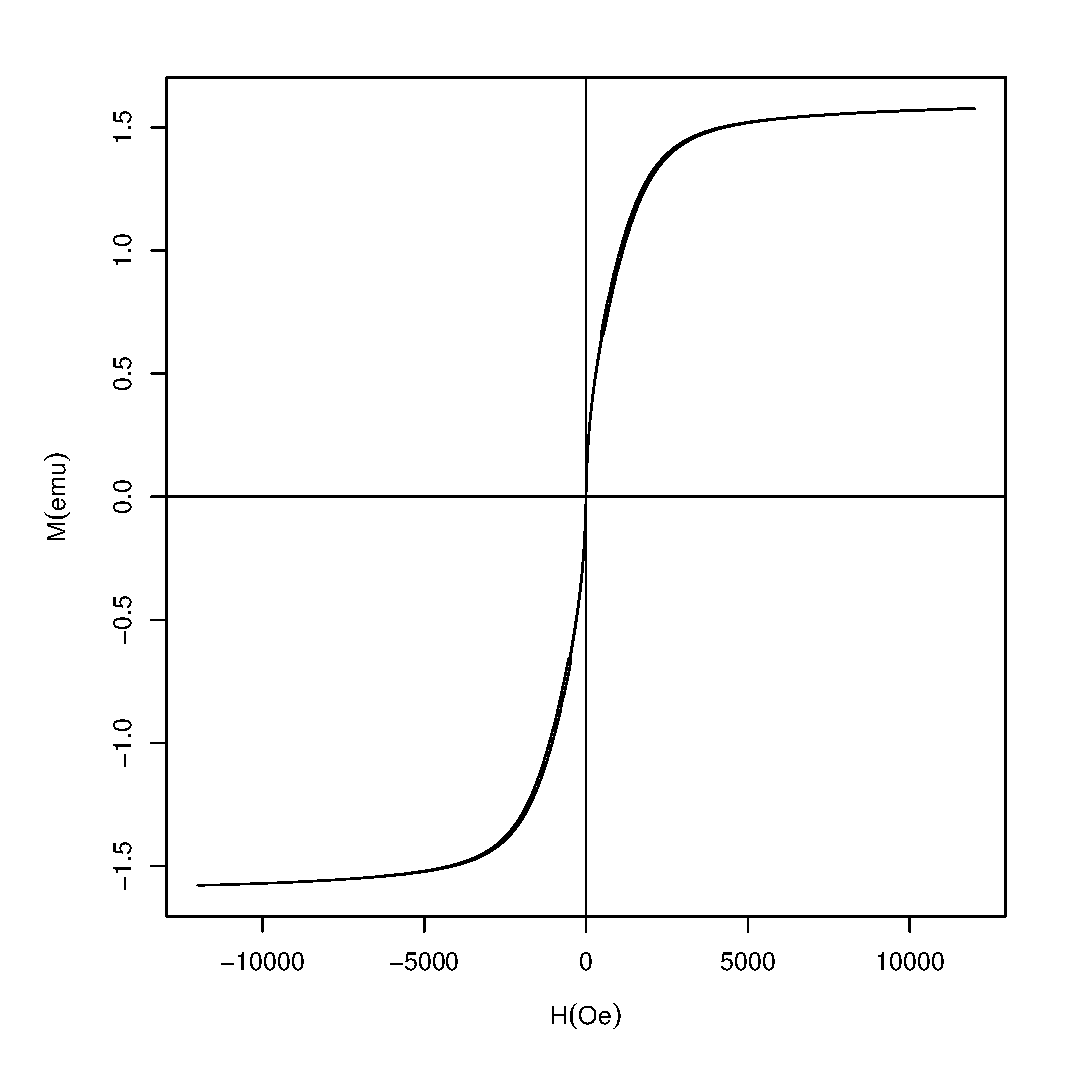
\includegraphics[width=125mm]{MagCharMCF_cgs.eps}
    \end{center}
    \caption{MCF H-Mループcgs単位系}
    \label{fig:MCF_cgs}
  \end{figure}

  \begin{figure}[htb]
    \begin{center}
      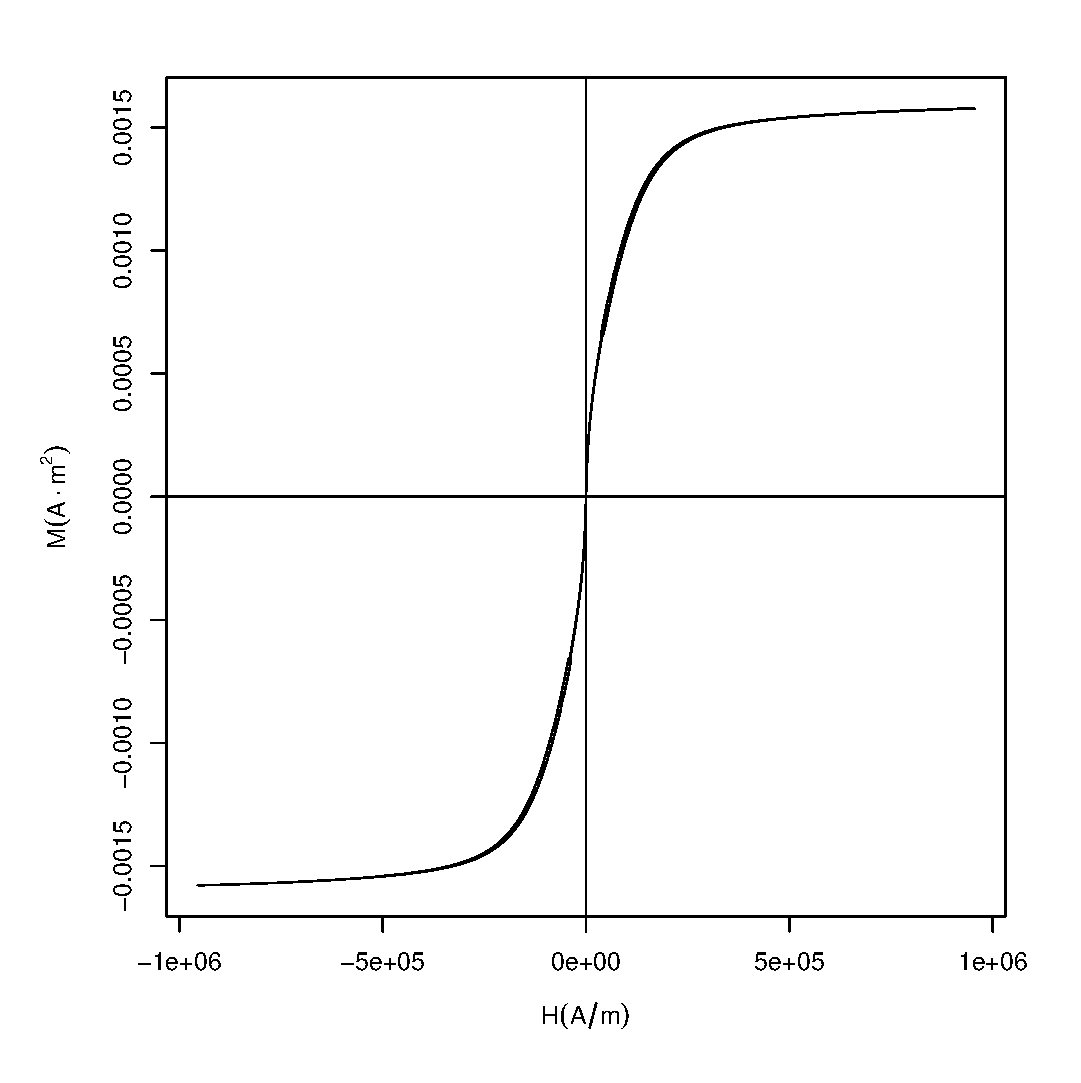
\includegraphics[width=125mm]{MagCharMCF_SI.eps}
    \end{center}
    \caption{MCF H-MループSI単位系}
    \label{fig:MCF_SI}
  \end{figure}

  \begin{figure}[htb]
    \begin{center}
      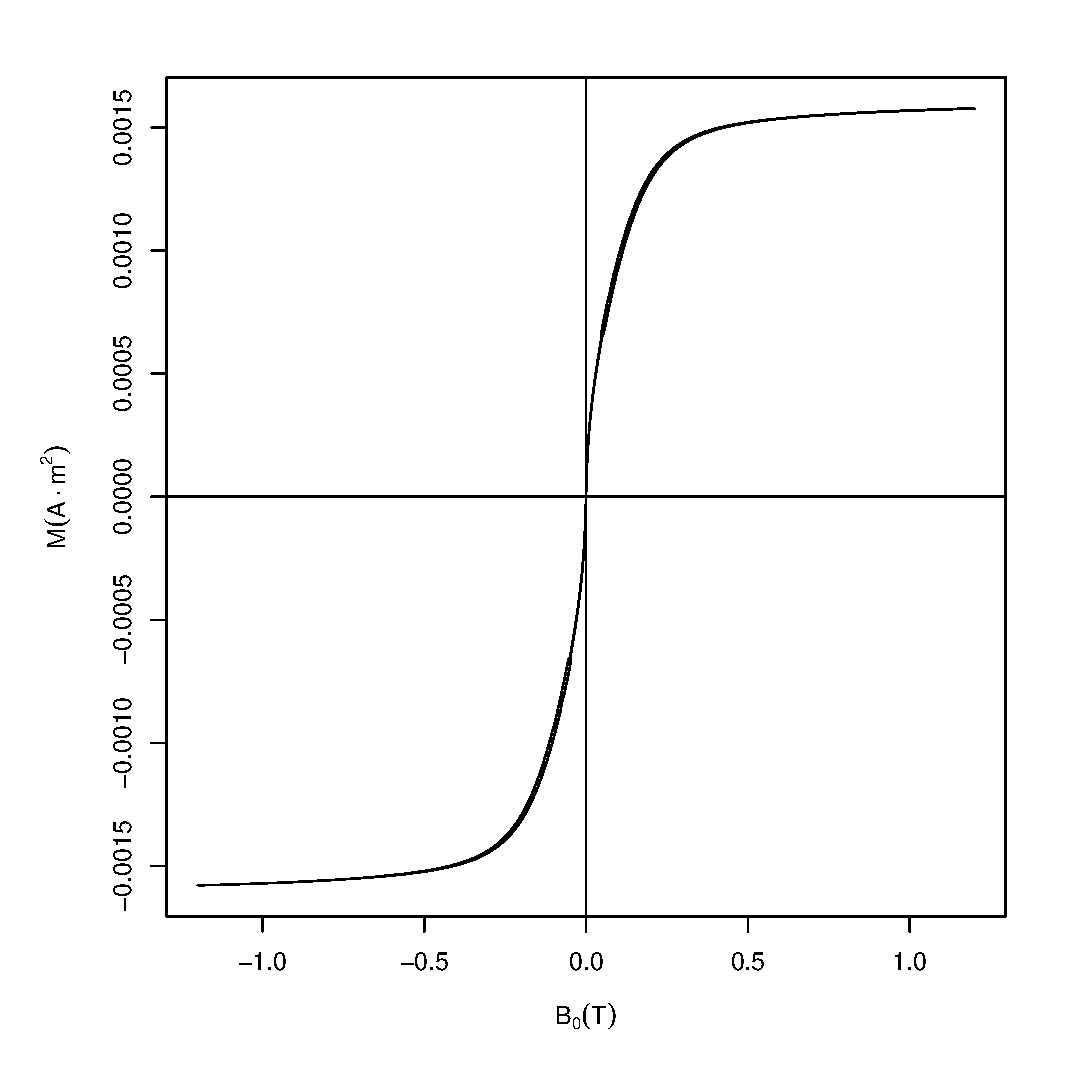
\includegraphics[width=125mm]{aaa.eps}
    \end{center}
    \caption{MCF B-MループSI単位系}
    \label{fig:MCF_SI_BM}
  \end{figure}

  \begin{figure}[htb]
    \begin{center}
      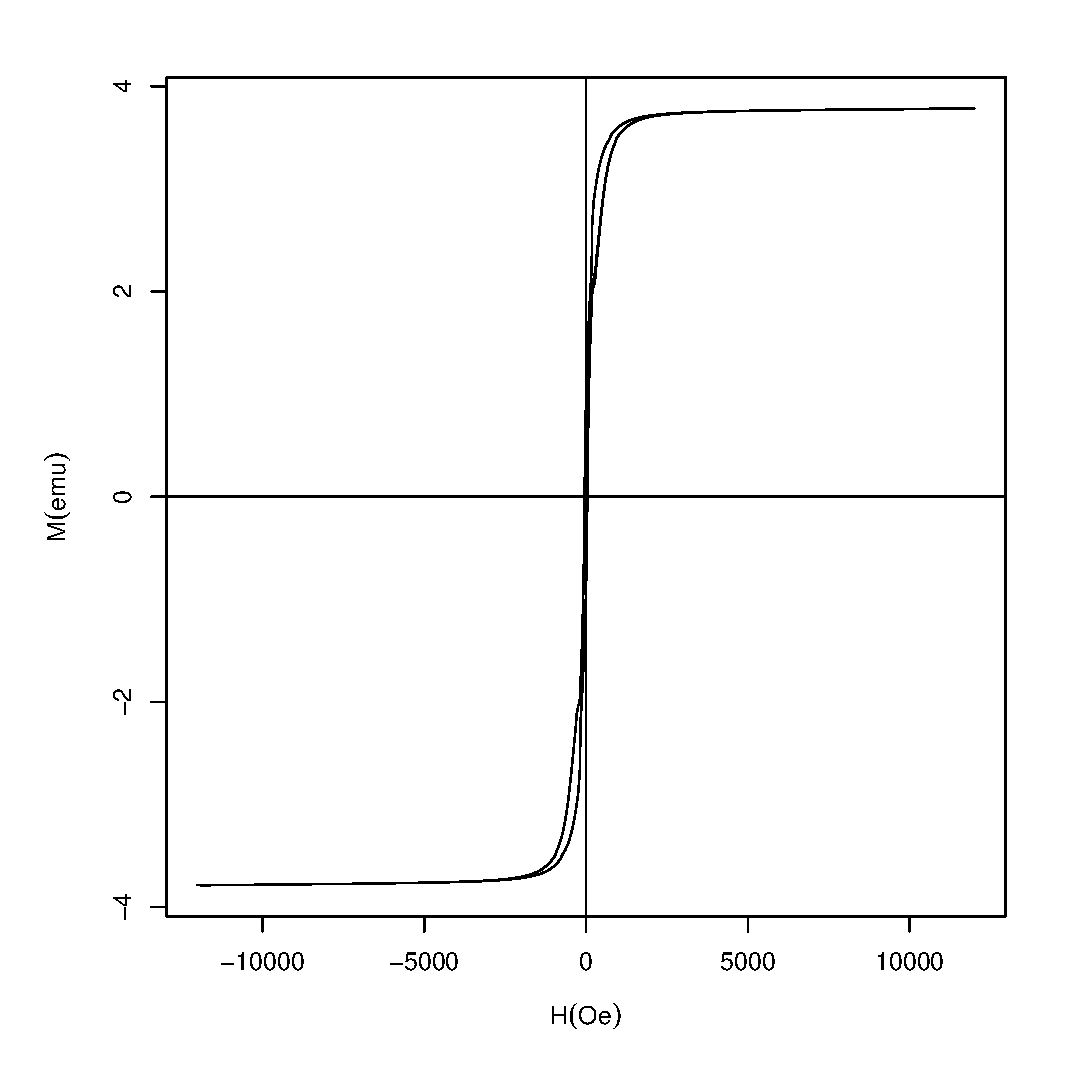
\includegraphics[width=125mm]{MagCharNi_cgs.eps}
    \end{center}
    \caption{Ni H-Mループcgs単位系}
    \label{fig:Ni_cgs}
  \end{figure}

  \begin{figure}[htb]
    \begin{center}
      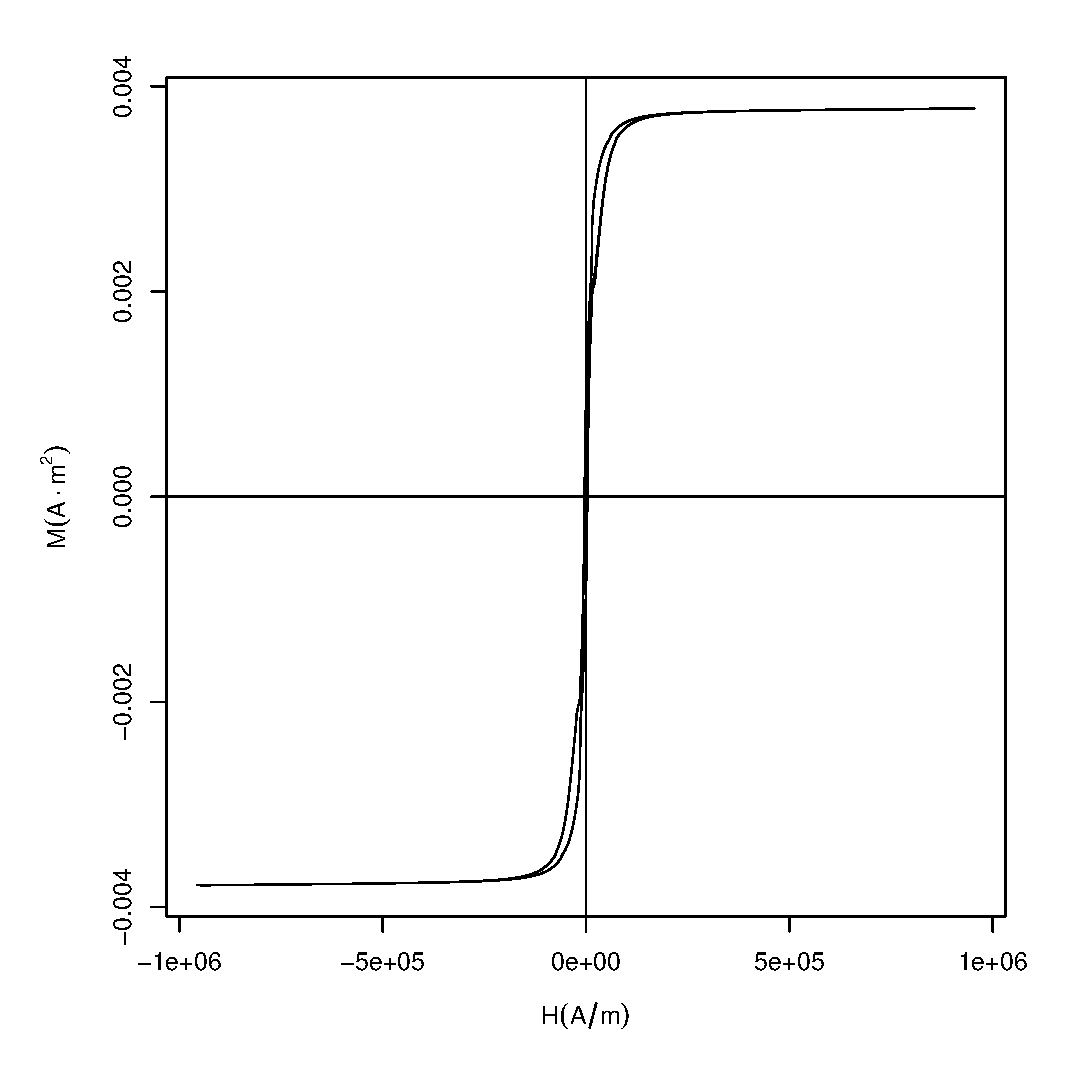
\includegraphics[width=125mm]{MagCharNi_SI.eps}
    \end{center}
    \caption{Ni H-MループSI単位系}
    \label{fig:Ni_SI}
  \end{figure}


\end{document}
